%%
%DIF LATEXDIFF DIFFERENCE FILE
%DIF DEL report-poster.tex   Sun Nov  5 22:14:21 2023
%DIF ADD kaggle-poster.tex   Wed Nov 29 15:08:53 2023
%% This is file `tikzposter-template.tex',
%% generated with the docstrip utility.
%%
%% The original source files were:
%%
%% tikzposter.dtx  (with options: `tikzposter-template.tex')
%%
%% This is a generated file.
%%
%% Copyright (C) 2014 by Pascal Richter, Elena Botoeva, Richard Barnard, and Dirk Surmann
%%
%% This file may be distributed and/or modified under the
%% conditions of the LaTeX Project Public License, either
%% version 2.0 of this license or (at your option) any later
%% version. The latest version of this license is in:
%%
%% http://www.latex-project.org/lppl.txt
%%
%% and version 2.0 or later is part of all distributions of
%% LaTeX version 2013/12/01 or later.
%%


\documentclass{tikzposter} %Options for format can be included here

\usepackage{todonotes}

\usepackage[tikz]{bclogo}
\usepackage{lipsum}
\usepackage{amsmath}

\usepackage{booktabs}
\usepackage{longtable}
\usepackage[absolute]{textpos}
\usepackage[it]{subfigure}
\usepackage{graphicx}
\usepackage{cmbright}
%\usepackage[default]{cantarell}
%\usepackage{avant}
%\usepackage[math]{iwona}
\usepackage[math]{kurier}
\usepackage[T1]{fontenc}


%% add your packages here
\usepackage{hyperref}
% for random text
\usepackage{lipsum}
\usepackage[english]{babel}
\usepackage[pangram]{blindtext}
%DIF 52a52
\usepackage{adjustbox} %DIF > 
%DIF -------

\colorlet{backgroundcolor}{blue!10}

 % Title, Author, Institute
\title{New York City Taxi Trip Duration}
\author{Tianjiao Wang}
\institute{Beijing Technology and Business University
}
%\titlegraphic{logos/tulip-logo.eps}

%Choose Layout
\usetheme{Wave}

%\definebackgroundstyle{samplebackgroundstyle}{
%\draw[inner sep=0pt, line width=0pt, color=red, fill=backgroundcolor!30!black]
%(bottomleft) rectangle (topright);
%}
%
%\colorlet{backgroundcolor}{blue!10}
%DIF PREAMBLE EXTENSION ADDED BY LATEXDIFF
%DIF UNDERLINE PREAMBLE %DIF PREAMBLE
\RequirePackage[normalem]{ulem} %DIF PREAMBLE
\RequirePackage{color}\definecolor{RED}{rgb}{1,0,0}\definecolor{BLUE}{rgb}{0,0,1} %DIF PREAMBLE
\providecommand{\DIFaddtex}[1]{{\protect\color{blue}\uwave{#1}}} %DIF PREAMBLE
\providecommand{\DIFdeltex}[1]{{\protect\color{red}\sout{#1}}}                      %DIF PREAMBLE
%DIF SAFE PREAMBLE %DIF PREAMBLE
\providecommand{\DIFaddbegin}{} %DIF PREAMBLE
\providecommand{\DIFaddend}{} %DIF PREAMBLE
\providecommand{\DIFdelbegin}{} %DIF PREAMBLE
\providecommand{\DIFdelend}{} %DIF PREAMBLE
\providecommand{\DIFmodbegin}{} %DIF PREAMBLE
\providecommand{\DIFmodend}{} %DIF PREAMBLE
%DIF FLOATSAFE PREAMBLE %DIF PREAMBLE
\providecommand{\DIFaddFL}[1]{\DIFadd{#1}} %DIF PREAMBLE
\providecommand{\DIFdelFL}[1]{\DIFdel{#1}} %DIF PREAMBLE
\providecommand{\DIFaddbeginFL}{} %DIF PREAMBLE
\providecommand{\DIFaddendFL}{} %DIF PREAMBLE
\providecommand{\DIFdelbeginFL}{} %DIF PREAMBLE
\providecommand{\DIFdelendFL}{} %DIF PREAMBLE
%DIF HYPERREF PREAMBLE %DIF PREAMBLE
\providecommand{\DIFadd}[1]{\texorpdfstring{\DIFaddtex{#1}}{#1}} %DIF PREAMBLE
\providecommand{\DIFdel}[1]{\texorpdfstring{\DIFdeltex{#1}}{}} %DIF PREAMBLE
\newcommand{\DIFscaledelfig}{0.5}
%DIF HIGHLIGHTGRAPHICS PREAMBLE %DIF PREAMBLE
\RequirePackage{settobox} %DIF PREAMBLE
\RequirePackage{letltxmacro} %DIF PREAMBLE
\newsavebox{\DIFdelgraphicsbox} %DIF PREAMBLE
\newlength{\DIFdelgraphicswidth} %DIF PREAMBLE
\newlength{\DIFdelgraphicsheight} %DIF PREAMBLE
% store original definition of \includegraphics %DIF PREAMBLE
\LetLtxMacro{\DIFOincludegraphics}{\includegraphics} %DIF PREAMBLE
\newcommand{\DIFaddincludegraphics}[2][]{{\color{blue}\fbox{\DIFOincludegraphics[#1]{#2}}}} %DIF PREAMBLE
\newcommand{\DIFdelincludegraphics}[2][]{% %DIF PREAMBLE
\sbox{\DIFdelgraphicsbox}{\DIFOincludegraphics[#1]{#2}}% %DIF PREAMBLE
\settoboxwidth{\DIFdelgraphicswidth}{\DIFdelgraphicsbox} %DIF PREAMBLE
\settoboxtotalheight{\DIFdelgraphicsheight}{\DIFdelgraphicsbox} %DIF PREAMBLE
\scalebox{\DIFscaledelfig}{% %DIF PREAMBLE
\parbox[b]{\DIFdelgraphicswidth}{\usebox{\DIFdelgraphicsbox}\\[-\baselineskip] \rule{\DIFdelgraphicswidth}{0em}}\llap{\resizebox{\DIFdelgraphicswidth}{\DIFdelgraphicsheight}{% %DIF PREAMBLE
\setlength{\unitlength}{\DIFdelgraphicswidth}% %DIF PREAMBLE
\begin{picture}(1,1)% %DIF PREAMBLE
\thicklines\linethickness{2pt} %DIF PREAMBLE
{\color[rgb]{1,0,0}\put(0,0){\framebox(1,1){}}}% %DIF PREAMBLE
{\color[rgb]{1,0,0}\put(0,0){\line( 1,1){1}}}% %DIF PREAMBLE
{\color[rgb]{1,0,0}\put(0,1){\line(1,-1){1}}}% %DIF PREAMBLE
\end{picture}% %DIF PREAMBLE
}\hspace*{3pt}}} %DIF PREAMBLE
} %DIF PREAMBLE
\LetLtxMacro{\DIFOaddbegin}{\DIFaddbegin} %DIF PREAMBLE
\LetLtxMacro{\DIFOaddend}{\DIFaddend} %DIF PREAMBLE
\LetLtxMacro{\DIFOdelbegin}{\DIFdelbegin} %DIF PREAMBLE
\LetLtxMacro{\DIFOdelend}{\DIFdelend} %DIF PREAMBLE
\DeclareRobustCommand{\DIFaddbegin}{\DIFOaddbegin \let\includegraphics\DIFaddincludegraphics} %DIF PREAMBLE
\DeclareRobustCommand{\DIFaddend}{\DIFOaddend \let\includegraphics\DIFOincludegraphics} %DIF PREAMBLE
\DeclareRobustCommand{\DIFdelbegin}{\DIFOdelbegin \let\includegraphics\DIFdelincludegraphics} %DIF PREAMBLE
\DeclareRobustCommand{\DIFdelend}{\DIFOaddend \let\includegraphics\DIFOincludegraphics} %DIF PREAMBLE
\LetLtxMacro{\DIFOaddbeginFL}{\DIFaddbeginFL} %DIF PREAMBLE
\LetLtxMacro{\DIFOaddendFL}{\DIFaddendFL} %DIF PREAMBLE
\LetLtxMacro{\DIFOdelbeginFL}{\DIFdelbeginFL} %DIF PREAMBLE
\LetLtxMacro{\DIFOdelendFL}{\DIFdelendFL} %DIF PREAMBLE
\DeclareRobustCommand{\DIFaddbeginFL}{\DIFOaddbeginFL \let\includegraphics\DIFaddincludegraphics} %DIF PREAMBLE
\DeclareRobustCommand{\DIFaddendFL}{\DIFOaddendFL \let\includegraphics\DIFOincludegraphics} %DIF PREAMBLE
\DeclareRobustCommand{\DIFdelbeginFL}{\DIFOdelbeginFL \let\includegraphics\DIFdelincludegraphics} %DIF PREAMBLE
\DeclareRobustCommand{\DIFdelendFL}{\DIFOaddendFL \let\includegraphics\DIFOincludegraphics} %DIF PREAMBLE
%DIF COLORLISTINGS PREAMBLE %DIF PREAMBLE
\RequirePackage{listings} %DIF PREAMBLE
\RequirePackage{color} %DIF PREAMBLE
\lstdefinelanguage{DIFcode}{ %DIF PREAMBLE
%DIF DIFCODE_UNDERLINE %DIF PREAMBLE
  moredelim=[il][\color{red}\sout]{\%DIF\ <\ }, %DIF PREAMBLE
  moredelim=[il][\color{blue}\uwave]{\%DIF\ >\ } %DIF PREAMBLE
} %DIF PREAMBLE
\lstdefinestyle{DIFverbatimstyle}{ %DIF PREAMBLE
	language=DIFcode, %DIF PREAMBLE
	basicstyle=\ttfamily, %DIF PREAMBLE
	columns=fullflexible, %DIF PREAMBLE
	keepspaces=true %DIF PREAMBLE
} %DIF PREAMBLE
\lstnewenvironment{DIFverbatim}{\lstset{style=DIFverbatimstyle}}{} %DIF PREAMBLE
\lstnewenvironment{DIFverbatim*}{\lstset{style=DIFverbatimstyle,showspaces=true}}{} %DIF PREAMBLE
%DIF END PREAMBLE EXTENSION ADDED BY LATEXDIFF

\begin{document}


\colorlet{blocktitlebgcolor}{blue!23}

 % Title block with title, author, logo, etc.
\maketitle

\begin{columns}
 % FIRST column
\column{0.5}% Width set relative to text width

%%%%%%%%%% -------------------------------------------------------------------- %%%%%%%%%%
 %\block{Main Objectives}{
%  	      	\begin{enumerate}
%  	      	\item Formalise research problem by extending \emph{outlying aspects mining}
%  	      	\item Proposed \emph{GOAM} algorithm is to solve research problem
%  	      	\item Utilise pruning strategies to reduce time complexity
%  	      	\end{enumerate}
%%  	      \end{minipage}
%}
%%%%%%%%%% -------------------------------------------------------------------- %%%%%%%%%%


%%%%%%%%%% -------------------------------------------------------------------- %%%%%%%%%%
\DIFdelbegin %DIFDELCMD < \block{Introduction}{
%DIFDELCMD <     The project will build a model that predicts the total ride duration of taxi trips in New York City. 
%DIFDELCMD <     The primary dataset is one released by the NYC Taxi and Limousine Commission, which includes pickup time, geo-coordinates, number of passengers, and several other variables.
%DIFDELCMD <     Accordingly,
%DIFDELCMD <     this project problem is 
%DIFDELCMD <     \emph{taxi trips duration},
%DIFDELCMD <     which is a \emph{outlier detection}.
%DIFDELCMD <   	

%DIFDELCMD <   	\begin{description}
\begin{description}%DIFAUXCMD
%DIFDELCMD <   	\item[Data cleaning ] aims to identify duplicated and missing values, and deal with outliers.
%DIFDELCMD <   	

%DIFDELCMD <   	\item[Features engineering] aims to visualize the distribution of trip-duration values, deal with categorical features, deal with dates, create distance and speed, do correlations and dimensionality reductions.
%DIFDELCMD <   	

%DIFDELCMD <   

\end{description}%DIFAUXCMD
%DIFDELCMD <   	\end{description}
%DIFDELCMD < 

%DIFDELCMD <   	In this paper,
%DIFDELCMD <     we extend the task of \emph{outlying aspects mining} to the \emph{group} level,
%DIFDELCMD <     formalize the research problem of \emph{group outlying aspects mining},
%DIFDELCMD <     and propose a novel algorithm named GOAM to solve the
%DIFDELCMD <     \emph{group outlying aspects mining} problem.
%DIFDELCMD < }
%DIFDELCMD < %%%
\DIFdelend \DIFaddbegin \block{Introduction}{
    The project will build a model that predicts the total ride duration of taxi trips in New York City. 
    The primary dataset is one released by the NYC Taxi and Limousine Commission, which includes pickup time, geo-coordinates, number of passengers, and several other variables.
    Accordingly, this project problem is \emph{taxi trips duration}, which is a \emph{outlier detection}.

  	\begin{description}
  	\item[\DIFadd{Data loading and overview }] aims to Loading the data and take a overview of the data.

  	\item[\DIFadd{Data cleaning }] aims to identify duplicated and missing values, and deal with outliers.

  	\item[\DIFadd{Features engineering}] aims to visualize the distribution of trip-duration values, deal with categorical features, deal with dates, create distance and speed, do correlations and dimensionality reductions.

  
  	\end{description}

  	This project  can predict the duration of each trip in the \emph{test set} , after \emph{model selecting},
    and  \emph{Hyperparameters tuning} .
}
\DIFaddend %%%%%%%%%% -------------------------------------------------------------------- %%%%%%%%%%


%%%%%%%%%% -------------------------------------------------------------------- %%%%%%%%%%
\DIFdelbegin %DIFDELCMD < \block{Group Outlying Aspects Mining}{
%DIFDELCMD < \begin{itemize}
\begin{itemize}%DIFAUXCMD
%DIFDELCMD <     \item
\item%DIFAUXCMD
%DIFDELCMD <     %\emph{Group Outlying Aspects Mining}
%DIFDELCMD <     It aims to \emph{identify a subset of aspects (or subspace)
%DIFDELCMD <     which makes the query group, rather than the single object,
%DIFDELCMD <     obviously different}.
%DIFDELCMD <     What we are interested in the task of \emph{group outlying aspects mining}
%DIFDELCMD <     is to explain which aspects make the query group distinctive
%DIFDELCMD <     different from the other groups.
%DIFDELCMD < 

%DIFDELCMD <     \item
\item%DIFAUXCMD
%DIFDELCMD <     \emph{Group Outlying Aspects Mining},
%DIFDELCMD <     \emph{Outlying Aspects Mining} and
%DIFDELCMD <     \emph{Outlier Detection} are different with each other.

\end{itemize}%DIFAUXCMD
%DIFDELCMD < \end{itemize}
%DIFDELCMD < 

%DIFDELCMD < \begin{center}
%DIFDELCMD <     \begin{minipage}{0.3\linewidth}
%DIFDELCMD <     \centering
%DIFDELCMD <     \begin{tikzfigure}
%DIFDELCMD <     \missingfigure[figcolor=white]{Testing figcolor}
%DIFDELCMD <     {\small{Group Outlying Aspects Mining}}
%DIFDELCMD <     \end{tikzfigure}%
%DIFDELCMD <     \end{minipage}
%DIFDELCMD <     \hfill
%DIFDELCMD <     \begin{minipage}{0.3\linewidth}
%DIFDELCMD <     \centering
%DIFDELCMD <     \begin{tikzfigure}
%DIFDELCMD <     \missingfigure[figcolor=white]{Testing figcolor}
%DIFDELCMD <     {\small{Outlying Aspects Mining}}
%DIFDELCMD <     \end{tikzfigure}%
%DIFDELCMD <     \end{minipage}
%DIFDELCMD <     \hfill
%DIFDELCMD <     \begin{minipage}{0.3\linewidth}
%DIFDELCMD <     \centering
%DIFDELCMD <     \begin{tikzfigure}
%DIFDELCMD <     \missingfigure[figcolor=white]{Testing figcolor}
%DIFDELCMD <     {\small{Outlier Detection}}
%DIFDELCMD <     \end{tikzfigure}%
%DIFDELCMD <     \end{minipage}
%DIFDELCMD < \end{center}
%DIFDELCMD < }
%DIFDELCMD < %%%
\DIFdelend \DIFaddbegin \block{Data loading and overview}{
\begin{itemize}
    \item
    %\emph{Data loading and overview}
    At first, I \emph{quickly look at the first 5 lines of a dataset to understand the structure, format, and content of the data }.
    Then I take a overview of \emph{the type and amount and other information of df and test data}. 

%\item
%\emph{Group Outlying Aspects Mining},
%\emph{Outlying Aspects Mining} and
%\emph{Outlier Detection} are different with each other.
\end{itemize}

\begin{center}
    \begin{minipage}{0.3\linewidth}
    \centering
%    \begin{tikzfigure}
%    \missingfigure[figcolor=white]{Testing figcolor}
%    {\small{Group Outlying Aspects Mining}}
%    \end{tikzfigure}%
    \end{minipage}
    \hfill
    \begin{minipage}{0.3\linewidth}
    \centering
    \begin{tikzfigure}
    \begin{adjustbox}{right=15cm}
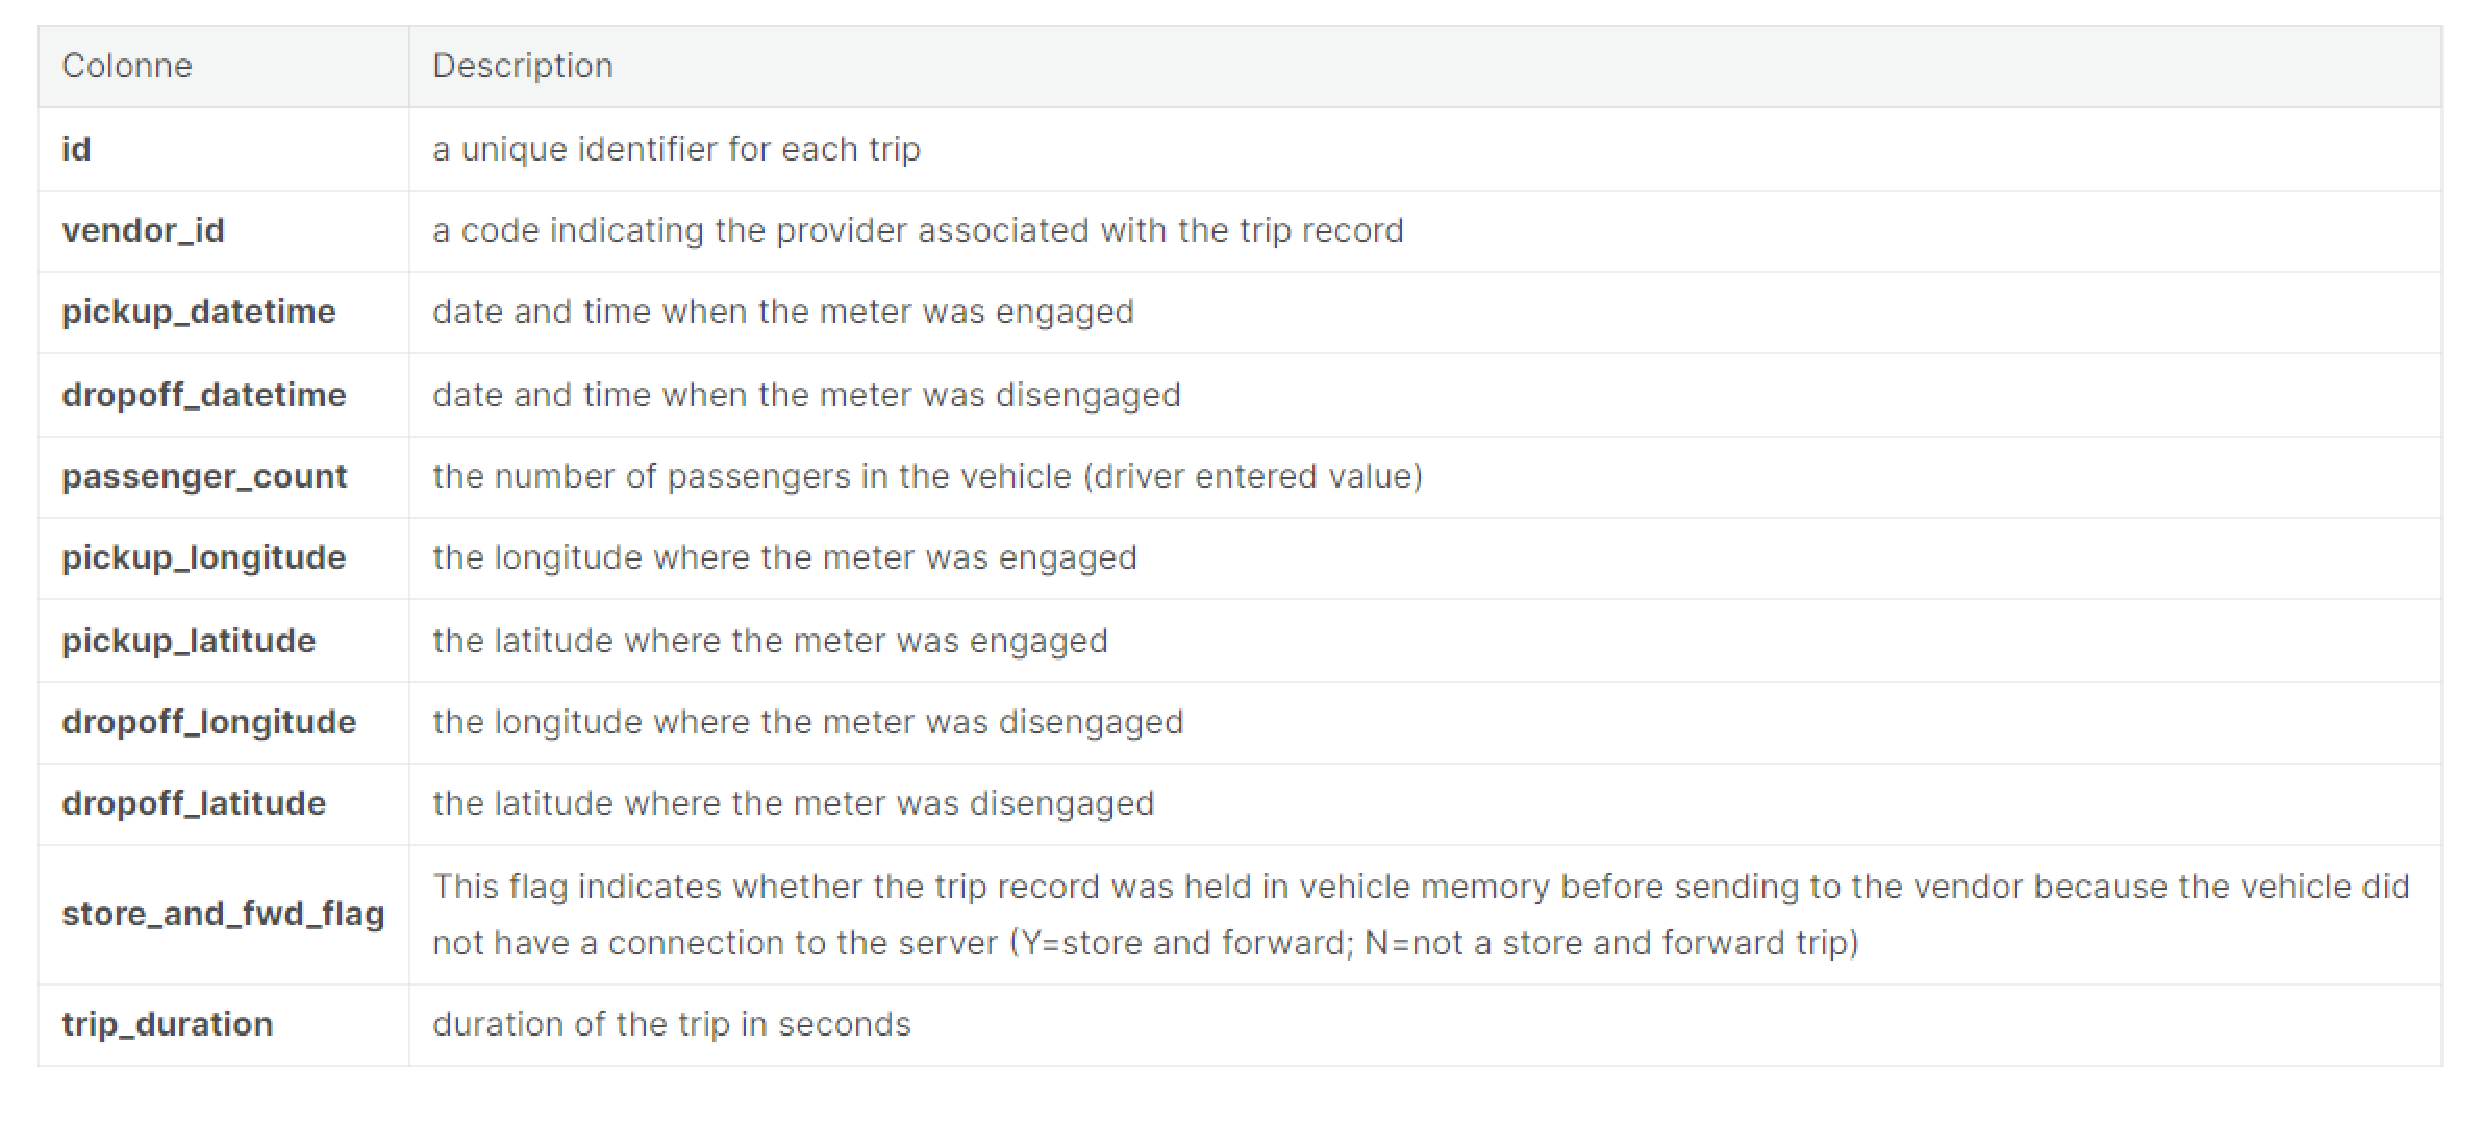
\includegraphics{E:/my study/BTBU Tourism/Flip00/Flip00-Tianjiao/templatex-develop/templatex/overview.eps}
    \end{adjustbox}
    {\small{overview of data}}
    \end{tikzfigure}%
    \end{minipage}
    \hfill
    \begin{minipage}{0.\linewidth}
    \centering
%    \begin{tikzfigure}
%    \missingfigure[figcolor=white]{Testing figcolor}
%    {\small{Outlier Detection}}
%    \end{tikzfigure}%
    \end{minipage}
\end{center}
}
\DIFaddend %%%%%%%%%% -------------------------------------------------------------------- %%%%%%%%%%


%%%%%%%%%% -------------------------------------------------------------------- %%%%%%%%%%

%\note{Note with default behavior}

%\note[targetoffsetx=12cm, targetoffsety=-1cm, angle=20, rotate=25]
%{Note \\ offset and rotated}

 % First column - second block


%%%%%%%%%% -------------------------------------------------------------------- %%%%%%%%%%
\DIFdelbegin %DIFDELCMD < \block{GOAM Algorithm}{
%DIFDELCMD <   	We propose the \emph{GOAM} algorithm to solve the research problem of
%DIFDELCMD <     \emph{Group Outlying Aspects Mining}.
%DIFDELCMD <   	The \emph{GOAM} algorithm includes three major steps.
%DIFDELCMD < %    1) Group Feature Extraction,
%DIFDELCMD < %    2) Outlying Degree Scoring, and
%DIFDELCMD < %    3) Outlying Aspects Identification.
%DIFDELCMD <   	

%DIFDELCMD < \begin{tikzfigure}%[Overall architecture of \emph{GOAM} algorithm]
%DIFDELCMD < %  \includegraphics[width=0.8\linewidth]{figures//framework.pdf}
%DIFDELCMD <     \missingfigure[figcolor=white]{Testing figcolor}
%DIFDELCMD < \end{tikzfigure}
%DIFDELCMD < 		

%DIFDELCMD < \begin{description}
\begin{description}%DIFAUXCMD
%DIFDELCMD <   	\item[Group Feature Extraction]
\item[\DIFdel{Group Feature Extraction}]%DIFAUXCMD
%DIFDELCMD <   	Let $f_1$, $f_2$, $f_3$ represent three features of $G_q$.
%DIFDELCMD <     We count the frequency of each value for one feature.
%DIFDELCMD <     Then use the histogram to represent each feature.
%DIFDELCMD <     Similarly,
%DIFDELCMD <     we can extract other features for each group.
%DIFDELCMD < 

%DIFDELCMD < %    \item
%DIFDELCMD < %    The histogram of $G_q$ on three features are as follows.

\end{description}%DIFAUXCMD
%DIFDELCMD < \end{description}
%DIFDELCMD < 

%DIFDELCMD < \begin{center}
%DIFDELCMD <     \begin{minipage}{0.3\linewidth}
%DIFDELCMD <     \centering
%DIFDELCMD <     \begin{tikzfigure}
%DIFDELCMD <     \missingfigure[figcolor=white]{Testing figcolor}
%DIFDELCMD <     {\small{Histogram of $G_q$ on $f_1$}}
%DIFDELCMD <     \end{tikzfigure}%
%DIFDELCMD <     \end{minipage}
%DIFDELCMD <     \hfill
%DIFDELCMD <     \begin{minipage}{0.3\linewidth}
%DIFDELCMD <     \centering
%DIFDELCMD <     \begin{tikzfigure}
%DIFDELCMD <     \missingfigure[figcolor=white]{Testing figcolor}
%DIFDELCMD <     {\small{Histogram of $G_q$ on $f_2$}}
%DIFDELCMD <     \end{tikzfigure}%
%DIFDELCMD <     \end{minipage}
%DIFDELCMD <     \hfill
%DIFDELCMD <     \begin{minipage}{0.3\linewidth}
%DIFDELCMD <     \centering
%DIFDELCMD <     \begin{tikzfigure}
%DIFDELCMD <     \missingfigure[figcolor=white]{Testing figcolor}
%DIFDELCMD <     {\small{Histogram of $G_q$ on $f_3$}}
%DIFDELCMD <     \end{tikzfigure}%
%DIFDELCMD <     \end{minipage}
%DIFDELCMD < \end{center}
%DIFDELCMD < \begin{description}
\begin{description}%DIFAUXCMD
%DIFDELCMD < \item[Outlying Degree Scoring]
\item[\DIFdel{Outlying Degree Scoring}]%DIFAUXCMD
%DIFDELCMD <     In this step,
%DIFDELCMD <     we first calculate the \emph{earth mover distance} (EMD) of one feature among different groups.
%DIFDELCMD <     The earth mover distance reflects the minimum mean distance
%DIFDELCMD <     between groups on one feature.
%DIFDELCMD <     So,
%DIFDELCMD <     we utilize the EMD to measure the difference between groups of each feature.

\end{description}%DIFAUXCMD
%DIFDELCMD < \end{description}
%DIFDELCMD < }
%DIFDELCMD < %%%
\DIFdelend \DIFaddbegin \block{Data cleaning }{
  	I do the \emph{data learning}  to check  the 
    \emph{duplicated and missing values} and \emph{deal with outliers }

%    1) Group Feature Extraction,
%    2) Outlying Degree Scoring, and
%    3) Outlying Aspects Identification.

\begin{tikzfigure}%[Overall architecture of \emph{GOAM} algorithm]
%  \includegraphics[width=0.8\linewidth]{figures//framework.pdf}
    \includegraphics{duplicate and missing.eps}
\end{tikzfigure}
\vspace{2cm}
\begin{description}
  	\item[\DIFadd{Visualize outliers}]

   There are outliers. I can't find a proper interpretation and it will probably damage our model, so I choose to get rid of them.

%    \item
%    The histogram of $G_q$ on three features are as follows.
\end{description}

\begin{center}
    \begin{minipage}{0.3\linewidth}
    \centering
    \begin{tikzfigure}
    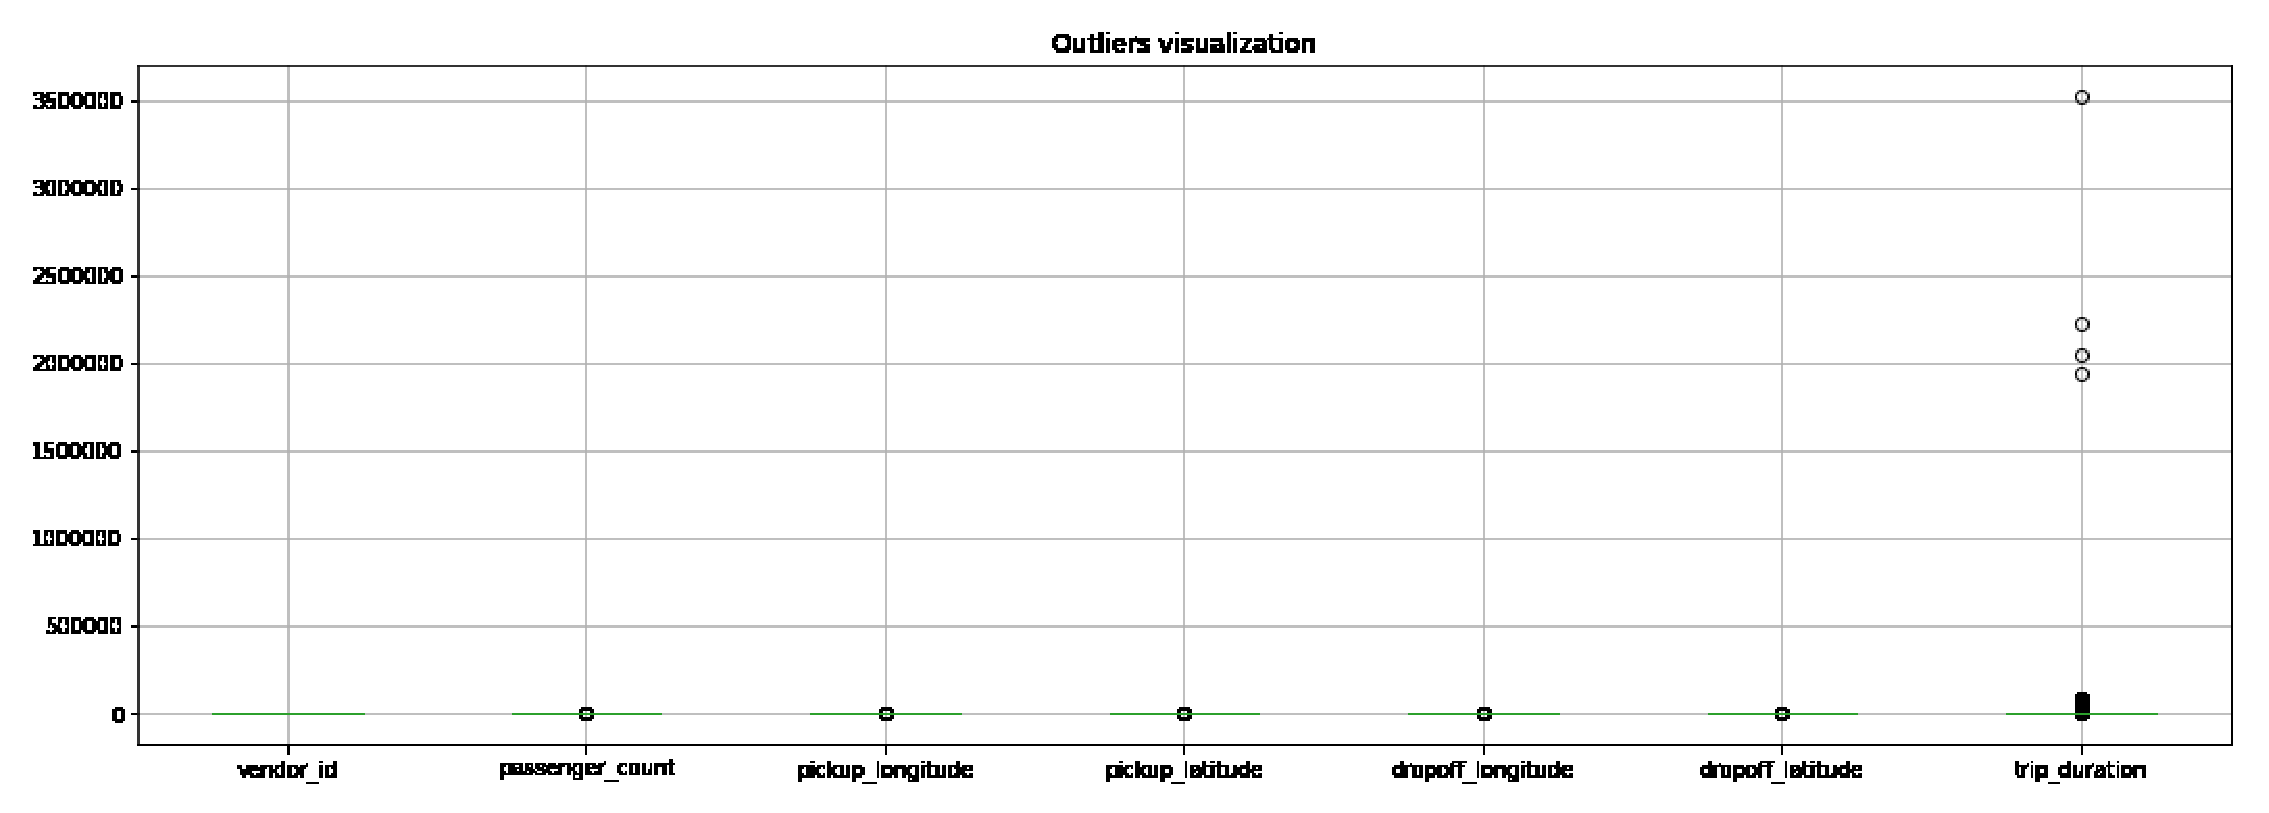
\includegraphics[scale=0.3]{outliers1.eps}
    {\small{outliers for trip-duration}}
    \end{tikzfigure}%
    \end{minipage}
    \hfill
    \begin{minipage}{0.3\linewidth}
    \centering
    \begin{tikzfigure}
    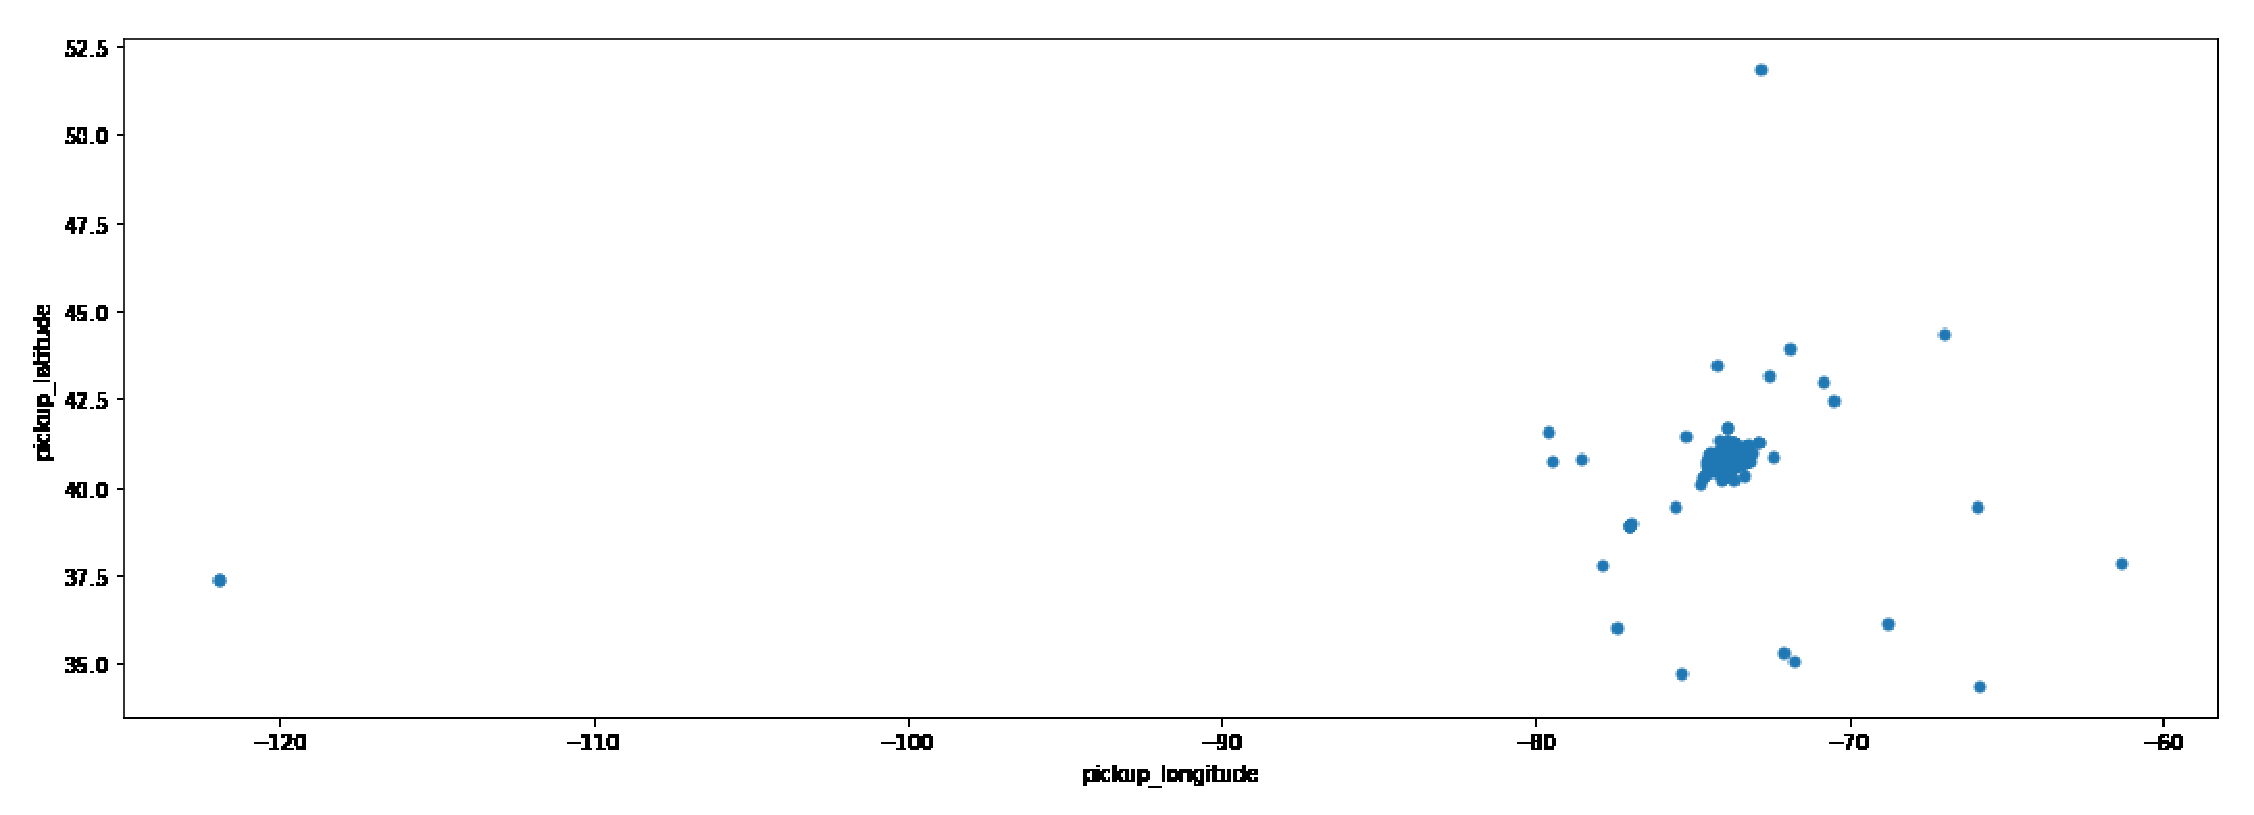
\includegraphics[scale=0.3]{outliers2.eps}
    {\small{outliers for pickup positions}}
    \end{tikzfigure}%
    \end{minipage}
    \hfill
    \begin{minipage}{0.3\linewidth}
    \centering
    \begin{tikzfigure}
   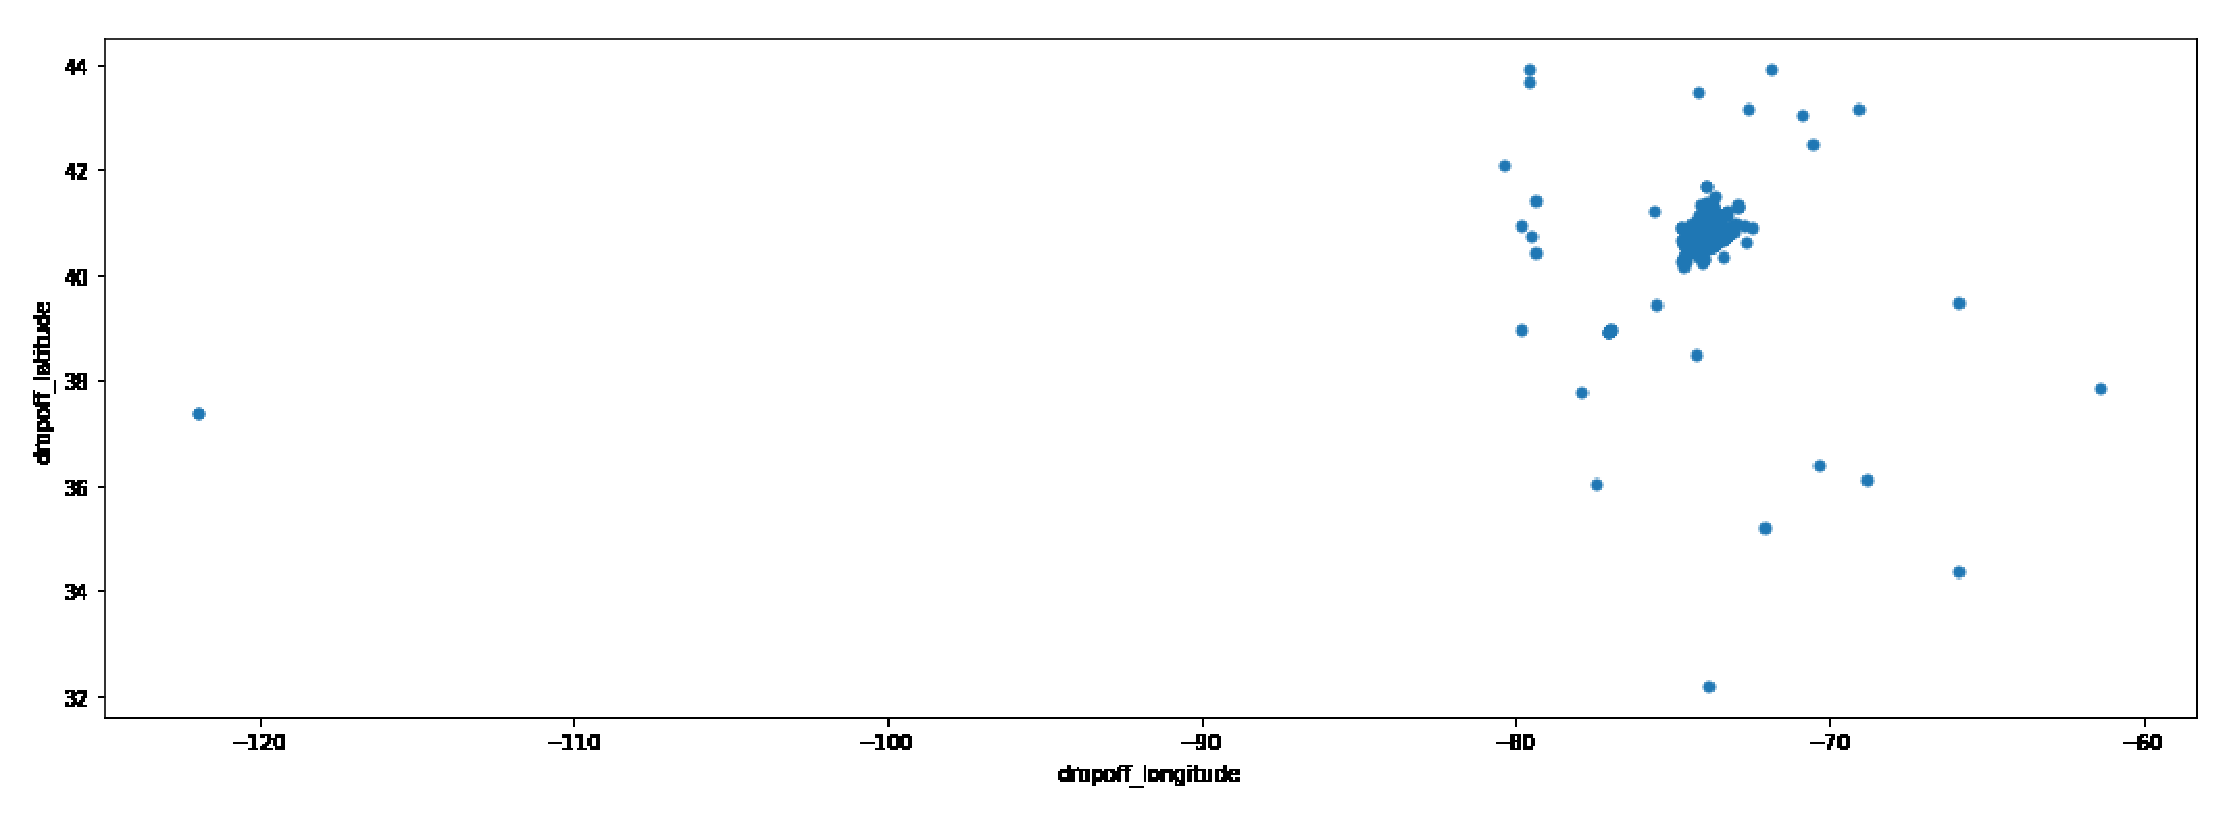
\includegraphics[scale=0.3]{outliers3.eps}
   {\small{outliers for dropoff positions}}
    \end{tikzfigure}%
    \end{minipage}
\end{center}
\begin{description}
\item[\DIFadd{visualize outliers}]

\vspace{2cm}
  \textit{ {\LARGE  In this step,
    I only keep trips that lasted less than 5900 seconds, and only keep trips with passengers.}}
\end{description}
}
\DIFaddend %%%%%%%%%% -------------------------------------------------------------------- %%%%%%%%%%


% SECOND column
\column{0.5}
 %Second column with first block's top edge aligned with with previous column's top.

%%%%%%%%%% -------------------------------------------------------------------- %%%%%%%%%%
\DIFdelbegin %DIFDELCMD < \block{GOAM Algorithm}{
%DIFDELCMD < \begin{description}
\begin{description}%DIFAUXCMD
%DIFDELCMD <     \item
\item%DIFAUXCMD
%DIFDELCMD <     Second,
%DIFDELCMD <     based on the \emph{earth move distance},
%DIFDELCMD <     we calculate the outlying degree.

\end{description}%DIFAUXCMD
%DIFDELCMD < \end{description}
%DIFDELCMD < 

%DIFDELCMD < \begin{tikzfigure}%[Overall architecture of \emph{GOAM} algorithm]
%DIFDELCMD <     \missingfigure[figcolor=white]{Testing figcolor}
%DIFDELCMD < \end{tikzfigure}
%DIFDELCMD <   where $G_q$ is the query group,
%DIFDELCMD <   $n$ is the number of compare groups,
%DIFDELCMD <   and $h_{k_s}$ is the histogram representation of $G_k$ in the subspace $s$.
%DIFDELCMD < 

%DIFDELCMD < \begin{description}
\begin{description}%DIFAUXCMD
%DIFDELCMD <   	\item[Outlying Aspects Identification]
\item[\DIFdel{Outlying Aspects Identification}]%DIFAUXCMD
%DIFDELCMD <     In this step,
%DIFDELCMD <     based on the value of outlying degree
%DIFDELCMD <     we will identify the group outlying aspects.
%DIFDELCMD <     If a feature's outlying degree is greater than a threshold,
%DIFDELCMD <     the more likely the feature is group outlying aspect.
%DIFDELCMD <     When the dimensionality of features is high,
%DIFDELCMD <     we adopt a stage-wise candidate subspace construction strategy to
%DIFDELCMD <     alleviate the exponential explosion.

\end{description}%DIFAUXCMD
%DIFDELCMD < \end{description}
%DIFDELCMD < }
%DIFDELCMD < %%%
\DIFdelend \DIFaddbegin \block{Features engineering}{
\begin{description}
    \item
    \emph{Visualize the distribution of trip-duration value},
\end{description}

\begin{tikzfigure}%[Overall architecture of \emph{GOAM} algorithm]
     \includegraphics[scale=0.9]{trip_duration.eps}
    {\small{The distribution of trip-duration values}}
\end{tikzfigure}
  The distribution is right-skewed so we can consider a log-transformation of trip-duration column.
  \item
  \emph{Deal with categorical features}
  \item
  \emph{Deal with dates}
  \item
  \emph{Distance and speed creations}
  \begin{tikzfigure}%[Overall architecture of \emph{GOAM} algorithm]
  	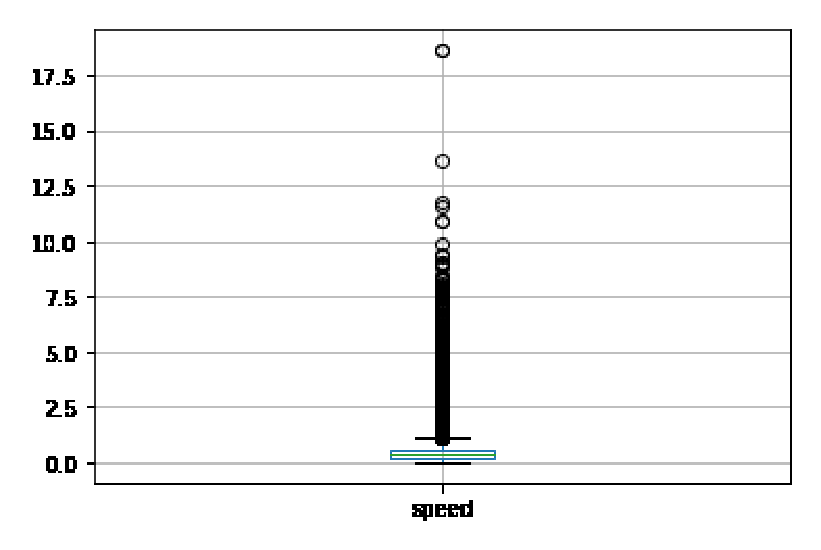
\includegraphics{speed.eps}
  	{\small{speed}}
  \end{tikzfigure}
  \item
  \emph{Correlations and dimensionality reductions}
  \begin{tikzfigure}%[Overall architecture of \emph{GOAM} algorithm]
  	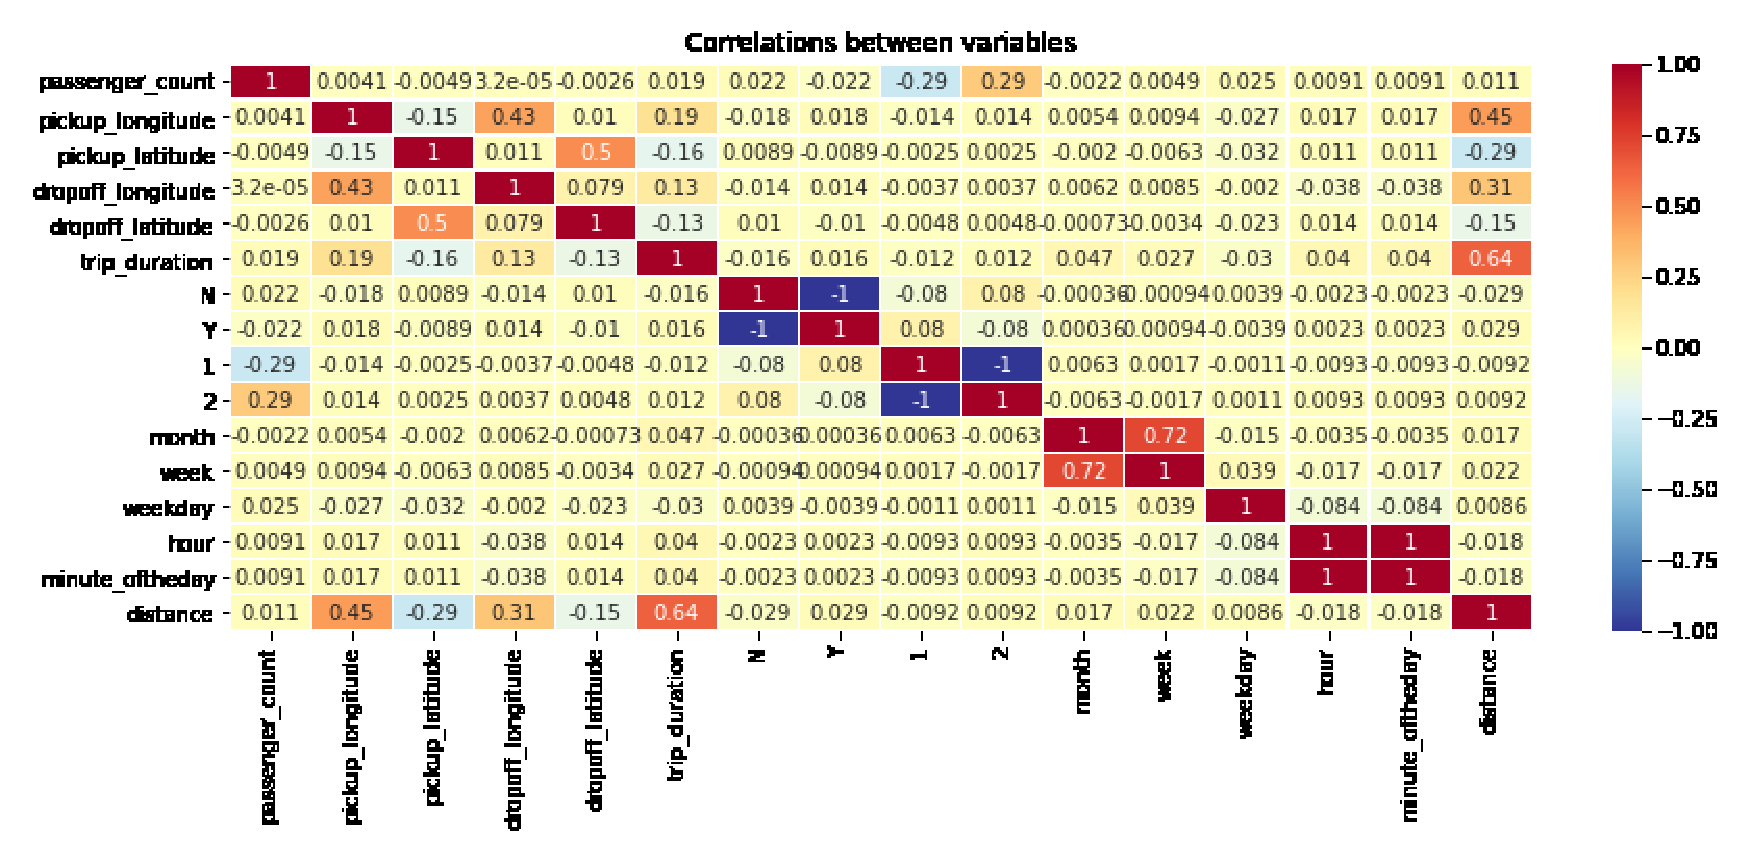
\includegraphics{correlations between variables.eps}
  	{\small{correlations between variables}}
  \end{tikzfigure}

%\begin{description}
%  	\item[\DIFadd{Outlying Aspects Identification}]
%    In this step,
%    based on the value of outlying degree
%    we will identify the group outlying aspects.
%    If a feature's outlying degree is greater than a threshold,
%    the more likely the feature is group outlying aspect.
%    When the dimensionality of features is high,
%    we adopt a stage-wise candidate subspace construction strategy to
%    alleviate the exponential explosion.
%\end{description}
}
\DIFaddend %%%%%%%%%% -------------------------------------------------------------------- %%%%%%%%%%
% Second column - first block


%%%%%%%%%% -------------------------------------------------------------------- %%%%%%%%%%
\DIFdelbegin %DIFDELCMD < \block[titleleft]{Experiment}
%DIFDELCMD < %%%
\DIFdelend \DIFaddbegin \block[titleleft]{Model selection}
\DIFaddend {
\begin{description}
  	\DIFdelbegin %DIFDELCMD < \item[Synthetic Dataset] %%%
\item[\DIFdel{Synthetic Dataset}]%DIFAUXCMD
\DIFdel{contains $10$ groups and $8$ features.
    Each group consists of $10$ members, and each member has $8$ features. }%DIFDELCMD < \end{description}
%DIFDELCMD < \vspace{.5cm}
%DIFDELCMD < \begin{tabular}{ c | c | c | c }
%DIFDELCMD <     \toprule
%DIFDELCMD <     %%%
\DIFdel{Method     }%DIFDELCMD < &  %%%
\DIFdel{Truth Outlying Aspects    }%DIFDELCMD < & %%%
\DIFdel{Identified Aspects }%DIFDELCMD < & %%%
\DIFdel{Accuracy      }\DIFdelend \DIFaddbegin \item[\DIFadd{LightGBM}]  \DIFadd{is blazingly fast compared to RandomForest and classic GradientBoosting, while fitting better. It is our clear winner.}\DIFaddend \\
  	\DIFdelbegin %DIFDELCMD < \midrule
%DIFDELCMD <     %%%
\DIFdel{GOAM       }%DIFDELCMD < &  %%%
\DIFdel{$\{F_1\}$, $\{F_2F_4\}$   }%DIFDELCMD < &  %%%
\DIFdel{$\{F_1\}$, $\{F_2F_4\}$    }%DIFDELCMD < & %%%
\DIFdel{100\%    }%DIFDELCMD < \\
%DIFDELCMD < %%%
\DIFdelend 

  	\DIFdelbegin \DIFdel{Arithmetic Mean based OAM }%DIFDELCMD < &  %%%
\DIFdel{$\{F_1\}$, $\{F_2F_4\}$   }%DIFDELCMD < &  %%%
\DIFdel{$\{F_4\}$, $\{F_2\}$    }%DIFDELCMD < &  %%%
\DIFdel{0\% }%DIFDELCMD < \\
%DIFDELCMD < 

%DIFDELCMD <      %%%
\DIFdel{Median based OAM }%DIFDELCMD < &  %%%
\DIFdel{$\{F_1\}$, $\{F_2F_4\}$   }%DIFDELCMD < &  %%%
\DIFdel{$\{F_2\}$, $\{F_4\}$    }%DIFDELCMD < &           %%%
\DIFdel{0\% }%DIFDELCMD < \\
%DIFDELCMD <      \bottomrule
%DIFDELCMD < \end{tabular}
%DIFDELCMD < \vspace{.2cm}
%DIFDELCMD < \begin{description}
%DIFDELCMD <     \item
\item%DIFAUXCMD
%DIFDELCMD <     %%%
\DIFdel{It can be observed that the GOAM method can identify the trivial outlying features
    and non-trivial outlying subspaces correctly and is obvious from the table
    that the accuracy of GOAM is the best, which is ($100\%$).}\DIFdelend \DIFaddbegin \vspace{0.5cm}
  	\DIFadd{Our LightGBM model is stable.
}\DIFaddend \end{description}
\DIFdelbegin %DIFDELCMD < 

%DIFDELCMD < \begin{description}
\begin{description}%DIFAUXCMD
%DIFDELCMD < \item[NBA Dataset] %%%
\item[\DIFdel{NBA Dataset}]%DIFAUXCMD
\DIFdel{was collected from Yahoo Sports
website (}%DIFDELCMD < \url{http://sports.yahoo.com.cn/nba}%%%
\DIFdel{).
The data include all teams from the six divisions,
and each player in the team has $12$ features.
}
\end{description}%DIFAUXCMD
%DIFDELCMD < \end{description}
%DIFDELCMD < %%%
\DIFdelend \vspace{.5cm}
\DIFdelbegin %DIFDELCMD < \begin{tabular}{ c | c | c }
%DIFDELCMD <     \toprule
%DIFDELCMD <     %%%
\DIFdel{Teams                   }%DIFDELCMD < & %%%
\DIFdel{Trivial Outlying Aspects  }%DIFDELCMD < & %%%
\DIFdel{NonTrivial Outlying Aspects    }%DIFDELCMD < \\
%DIFDELCMD <     \toprule
%DIFDELCMD <     %%%
\DIFdel{Cleveland Cavaliers     }%DIFDELCMD < & %%%
\DIFdel{\{3FA\}                   }%DIFDELCMD < & %%%
\DIFdel{\{FGA, FT\%\}, \{FGA, FG\%\} }%DIFDELCMD < \\
%DIFDELCMD <     %%%
\DIFdel{Orlando Magic           }%DIFDELCMD < & %%%
\DIFdel{\{Stl\}                   }%DIFDELCMD < & %%%
\DIFdel{None                         }%DIFDELCMD < \\
%DIFDELCMD <     %%%
\DIFdel{Milwaukee Bucks         }%DIFDELCMD < & %%%
\DIFdel{\{To\}, \{FTA\}           }%DIFDELCMD < & %%%
\DIFdel{\{FGA, FTA\}, \{3FA, FTA\}     }%DIFDELCMD < \\
%DIFDELCMD < %%%
%DIF <     Golden State Warriors   & \{FG\%\}                  & \{FT\%, Blk\}, \{FGA, 3PT\%, FTA\}\\
%DIF <     Utah Jazz               & \{Blk\}                   & \{3FA, 3PT\%\}                    \\
    \DIFdel{New Orleans Pelicans    }%DIFDELCMD < & %%%
\DIFdel{\{FT\%\}, \{FTA\}         }%DIFDELCMD < & %%%
\DIFdel{\{FTA, Stl\}, \{FTA, To\}          }%DIFDELCMD < \\
%DIFDELCMD <     \bottomrule
%DIFDELCMD < \end{tabular}
%DIFDELCMD <            %%%
\DIFdelend %DIF > \begin{tabular}{ c | c | c | c }
%DIF >     \toprule
%DIF >     Method     &  Truth Outlying Aspects    & Identified Aspects & Accuracy      \\
%DIF >     \midrule
%DIF >     GOAM       &  $\{F_1\}$, $\{F_2F_4\}$   &  $\{F_1\}$, $\{F_2F_4\}$    & 100\%    \\
%DIF > 
%DIF >      Arithmetic Mean based OAM &  $\{F_1\}$, $\{F_2F_4\}$   &  $\{F_4\}$, $\{F_2\}$    &  0\% \\
%DIF > 
%DIF >      Median based OAM &  $\{F_1\}$, $\{F_2F_4\}$   &  $\{F_2\}$, $\{F_4\}$    &           0\% \\
%DIF >      \bottomrule
%DIF > \end{tabular}
%DIF > \vspace{.2cm}
%DIF > \begin{description}
%DIF >     \item
%DIF >     It can be observed that the GOAM method can identify the trivial outlying features
%DIF >     and non-trivial outlying subspaces correctly and is obvious from the table
%DIF >     that the accuracy of GOAM is the best, which is ($100\%$).
%DIF > \end{description}
%DIF > 
%DIF > \begin{description}
%DIF > \item[NBA Dataset] was collected from Yahoo Sports
%DIF > website (\url{http://sports.yahoo.com.cn/nba}).
%DIF > The data include all teams from the six divisions,
%DIF > and each player in the team has $12$ features.
%DIF > \end{description}
%DIF > \vspace{.5cm}
%DIF > \begin{tabular}{ c | c | c }
%DIF >     \toprule
%DIF >     Teams                   & Trivial Outlying Aspects  & NonTrivial Outlying Aspects    \\
%DIF >     \toprule
%DIF >     Cleveland Cavaliers     & \{3FA\}                   & \{FGA, FT\%\}, \{FGA, FG\%\} \\
%DIF >     Orlando Magic           & \{Stl\}                   & None                         \\
%DIF >     Milwaukee Bucks         & \{To\}, \{FTA\}           & \{FGA, FTA\}, \{3FA, FTA\}     \\
%DIF > %    Golden State Warriors   & \{FG\%\}                  & \{FT\%, Blk\}, \{FGA, 3PT\%, FTA\}\\
%DIF > %    Utah Jazz               & \{Blk\}                   & \{3FA, 3PT\%\}                    \\
%DIF >     New Orleans Pelicans    & \{FT\%\}, \{FTA\}         & \{FTA, Stl\}, \{FTA, To\}          \\
%DIF >     \bottomrule
%DIF > \end{tabular}

\begin{minipage}{0.5\linewidth}
    \centering
\DIFdelbegin %DIFDELCMD < \begin{tikzfigure}
%DIFDELCMD <     \missingfigure[figcolor=white]{Testing figcolor}
%DIFDELCMD < 

%DIFDELCMD <     {\small{New Orleans Pelicans on FT\%}}
%DIFDELCMD <     \end{tikzfigure}%%%
\DIFdelend %DIF >     \begin{tikzfigure}
%DIF >     \missingfigure[figcolor=white]{Testing figcolor}
%
%DIF >     {\small{New Orleans Pelicans on FT\%}}
%DIF >     \end{tikzfigure}%
\end{minipage}
\hfill
\begin{minipage}{0.5\linewidth}
    \centering
\DIFdelbegin %DIFDELCMD < \begin{tikzfigure}
%DIFDELCMD <     \missingfigure[figcolor=white]{Testing figcolor}
%DIFDELCMD < 

%DIFDELCMD <     {\small{New Orleans Pelicans on FTA}}
%DIFDELCMD <     \end{tikzfigure}%%%
\DIFdelend %DIF >     \begin{tikzfigure}
%DIF >     \missingfigure[figcolor=white]{Testing figcolor}
%
%DIF >     {\small{New Orleans Pelicans on FTA}}
%DIF >     \end{tikzfigure}%
\end{minipage}
\DIFdelbegin %DIFDELCMD < \vspace{.2cm}
%DIFDELCMD < \begin{description}
\begin{description}%DIFAUXCMD
%DIFDELCMD < \item
\item%DIFAUXCMD
%DIFDELCMD < %%%
\texttt{\DIFdel{New Orleans Pelicans}} %DIFAUXCMD
\DIFdel{has more players with
lower \{free throw percentage\}, \{free throws attempted\}.
}
\end{description}%DIFAUXCMD
%DIFDELCMD < \end{description}
%DIFDELCMD < %%%
\DIFdelend %DIF > \vspace{.2cm}
%DIF > \begin{description}
%DIF > \item
%DIF > \texttt{New Orleans Pelicans} has more players with
%DIF > lower \{free throw percentage\}, \{free throws attempted\}.
%DIF > \end{description}
}
%%%%%%%%%% -------------------------------------------------------------------- %%%%%%%%%%


% Second column - second block
%%%%%%%%%% -------------------------------------------------------------------- %%%%%%%%%%
\block[titlewidthscale=1, bodywidthscale=1]
{\DIFdelbegin \DIFdel{Conclusion}\DIFdelend \DIFaddbegin \DIFadd{Training and predictions}\DIFaddend }
{
\begin{description}
  \DIFdelbegin %DIFDELCMD < \item[Problem Definition]
\item[\DIFdel{Problem Definition}]%DIFAUXCMD
%DIFDELCMD <   %%%
\DIFdel{Formalize the problem of Group Outlying Aspects Mining by extending outlying aspects mining.
}\DIFdelend \DIFaddbegin \item[\DIFadd{Training}]
  \DIFadd{Training on all labeled data using the best parameters
}\DIFaddend 

  \DIFdelbegin %DIFDELCMD < \item[GOAM algorithm]
\item[\DIFdel{GOAM algorithm}]%DIFAUXCMD
%DIFDELCMD <   %%%
\DIFdel{Propose GOAM algorithm to solve the }\emph{\DIFdel{Group}}%DIFAUXCMD
%DIFDELCMD < \\
%DIFDELCMD <   %%%
\emph{\DIFdel{Outlying Aspects Mining}} %DIFAUXCMD
\DIFdel{problem.
}%DIFDELCMD < 

%DIFDELCMD <   \item[Strategies]
\item[\DIFdel{Strategies}]%DIFAUXCMD
%DIFDELCMD <   %%%
\DIFdel{Utilize the pruning strategies to }%DIFDELCMD < \\ %%%
\DIFdel{reduce time complexity.
}\DIFdelend \DIFaddbegin \item[\DIFadd{Prediction}]
  \DIFadd{Make predictions on test data frame
  }\begin{tikzfigure}%DIF > [Overall architecture of \emph{GOAM} algorithm]
  	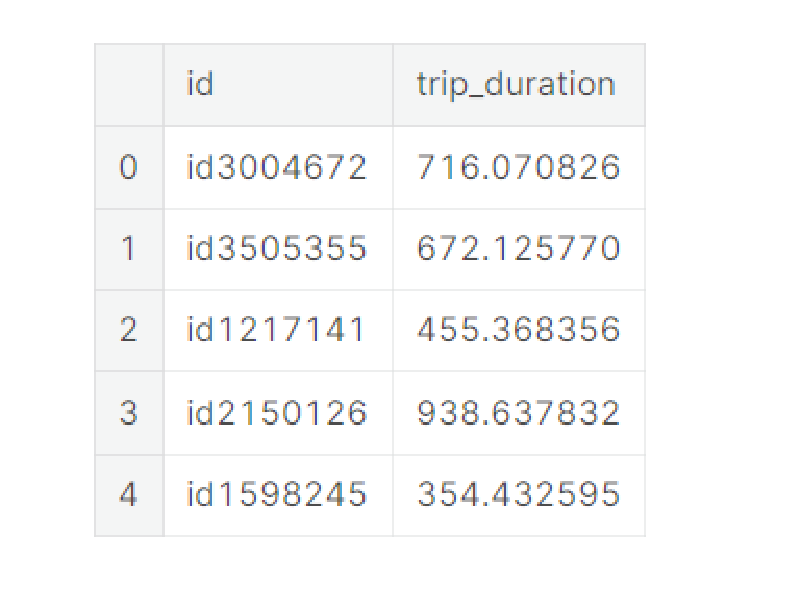
\includegraphics{predict_result.eps}
  	{\small{predict-result.eps}}
  \end{tikzfigure}
%DIF >   \item[\DIFadd{Strategies}]
%DIF >   Utilize the pruning strategies to \\ reduce time complexity.
\DIFaddend \end{description}
}
%%%%%%%%%% -------------------------------------------------------------------- %%%%%%%%%%


% Bottomblock
%%%%%%%%%% -------------------------------------------------------------------- %%%%%%%%%%
\colorlet{notebgcolor}{blue!20}
\colorlet{notefrcolor}{blue!20}
\DIFdelbegin %DIFDELCMD < \note[targetoffsetx=8cm, targetoffsety=-4cm, angle=30, rotate=15,
%DIFDELCMD < radius=2cm, width=.26\textwidth]{
%DIFDELCMD < Acknowledgement
%DIFDELCMD < \begin{itemize}
\begin{itemize}%DIFAUXCMD
%DIFDELCMD <     \item
\item%DIFAUXCMD
%DIFDELCMD <     International Cooperation Project (Y7Z0511101)
%DIFDELCMD <     of IIE,
%DIFDELCMD <     Chinese Academy of Sciences

\end{itemize}%DIFAUXCMD
%DIFDELCMD <  \end{itemize}
%DIFDELCMD < }
%DIFDELCMD < %%%
\DIFdelend \DIFaddbegin \note[targetoffsetx=8cm, targetoffsety=-4cm, angle=30, rotate=15,
radius=2cm, width=.26\textwidth]{
Acknowledgement
\begin{itemize}
    \item
    Flip00 learning-kaggle project
 \end{itemize}
}
\DIFaddend 

%\note[targetoffsetx=8cm, targetoffsety=-10cm,rotate=0,angle=180,radius=8cm,width=.46\textwidth,innersep=.1cm]{
%Acknowledgement
%}

%\block[titlewidthscale=0.9, bodywidthscale=0.9]
%{Acknowledgement}{
%}
%%%%%%%%%% -------------------------------------------------------------------- %%%%%%%%%%

\end{columns}


%%%%%%%%%% -------------------------------------------------------------------- %%%%%%%%%%
%[titleleft, titleoffsetx=2em, titleoffsety=1em, bodyoffsetx=2em,%
%roundedcorners=10, linewidth=0mm, titlewidthscale=0.7,%
%bodywidthscale=0.9, titlecenter]

%\colorlet{noteframecolor}{blue!20}
\colorlet{notebgcolor}{blue!20}
\colorlet{notefrcolor}{blue!20}
\note[targetoffsetx=-13cm, targetoffsety=-12cm,rotate=0,angle=180,radius=8cm,width=.96\textwidth,innersep=.4cm]
{
\begin{minipage}{0.3\linewidth}
\centering
\includegraphics[width=24cm]{./graphics/logos/tulip-wordmark.eps}
\end{minipage}
\begin{minipage}{0.7\linewidth}
{ \centering
 \DIFdelbegin \DIFdel{The $11^{th}$ International Conference on Knowledge Science, Engineering and Management (KSEM 2018),
  17-19/08/2018, Changchun}\DIFdelend \DIFaddbegin \DIFadd{Flip00-kaggle project, Beijing}\DIFaddend , China
}
\end{minipage}
}
%%%%%%%%%% -------------------------------------------------------------------- %%%%%%%%%%

\end{document}

%\endinput
%%
%% End of file `tikzposter-template.tex'.
